Our prototype has been written in Java and makes use of the REST API of Kubernetes. 
This component was initially a Java executable that operated outside a Kubernetes cluster,
but at the end it has been shipped inside a container using the building functionality of OpenFaas.
The testing will check two main characteristics: functional requirements and performance.  
\\
\subsubsection*{Functional Requirements}
\paragraph{}
First of all we needed to check if the Kubernetes API was reachable from our code.
The first executable was configured to access a cluster from outside. This was done by loading
the administrator configuration file in the API.
The limit of this method was that the component had to be launched on the administrator machine with a JVM
and that it had full control of the cluster. 
\\
These problems were solved by building a container with our executable by using OpenFaas and deploying it
in the cluster.
\\
In Kubernetes permissions are granted to pods by creating new Roles. These are objects that tell which API 
calls can be made by an agent inside the cluster, and can specify which objects can be affected by a call.
\\
Since a running pod does not have access to the old configuration file (because it's not deployed on the administrator machine),
it doesn't have the permission to read and updated nodes' labels, and so we had to link it to a Role.
After doing this procedure, the behavior of the component inside and outside the cluster is identical,
since it does not affect the SLPA code.
\paragraph{}
For what concerns SLPA, the algorithm in the container runs only if the nodes that
are given as input are registered inside the Kubernetes cluster. Since this check does not have
any effect on the execution of the algorithm and requires the presence of real hosts in a network,
we decided to unit-test the algorithm locally outside the container.
We created a dummy network (\ref{fig:RR2}) by filling the delay matrix and giving it to the algorithm.
The delay matrix is a  $NxN$ matrix, where N is the number of nodes of the network.
The cell M[$i$,$j$] contains the delay between the node $i$ and $j$. If this
cell is set to -1, there is no arc that links the two nodes. A delay threshold given as input will set to -1
all the cells that have a delay greater than that. In this example, the network shown is the one obtained after 
deleting all of these arcs that have a too high delay. The delays are not shown in the figure in order
to keep the visualization simple and because SLPA does not consider the value of the arcs but only their presence.
Note that in a real world scenario this delay would be measured for example by pinging the target node.
\par
Figure \ref{fig:netNoRR} shows the result of the algorithm without Round Robin. In this output the size of the 
different communities varies a lot. Since SLPA makes some decision based on chance, reapplying the
algorithm on the same network will give different results, creating each time different communities.
Figure \ref{fig:RR1} and \ref{fig:RR2} shows the effects of the Round Robin on the communities that were exceeding 
in size. In this examples, the maximum size of a community was set to 5. In figure \ref{fig:RR1} SLPA returned
two communities, one that included all the nodes from 1 to 8 while the other one included the remaining ones.
These were broken down  by the RR, creating 4 communities that cannot be broken down in 4 different partitions.
Figure \ref{fig:RR2} shows a luckier iteration of SLPA, that returned only one oversized community (from node 9
to node 15). 
\\
The fact that some nodes are not directly connected to the others of the same community is not a problem,
since sometimes also SLPA outputs communities with a structure similar to the one returned by the Round Robin in these examples.
However, if SLPA returns a very large community, with size much larger than the maximum size allowed, a set of communities
with disconnected nodes could be created, since there is no logic that tries to group closer nodes.
This result would be not optimal, since for sure exists another configuration that can have lower
overall delay between the nodes of a community.


\begin{figure}[]
    \centering
    \subfloat[Dummy Netowrk]{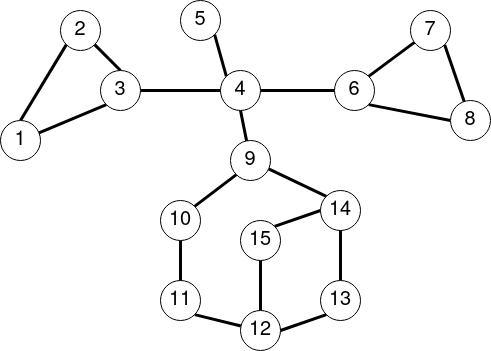
\includegraphics[width=.45\linewidth]{Images/rete.png}
    \label{fig:network}}
    \subfloat[SLPA without RR]{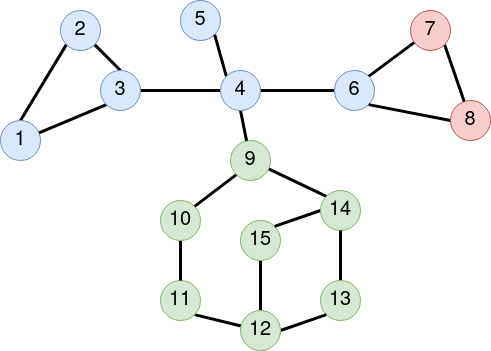
\includegraphics[width=.45\linewidth]{SLPAnoLimit.png}
    \label{fig:netNoRR}}
    \\
    \subfloat[SLPA with RR]{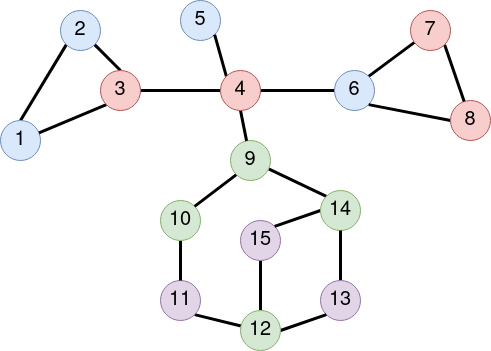
\includegraphics[width=.45\linewidth]{SLPARR5.png}
    \label{fig:RR1}}
    \subfloat[SLPA with RR]{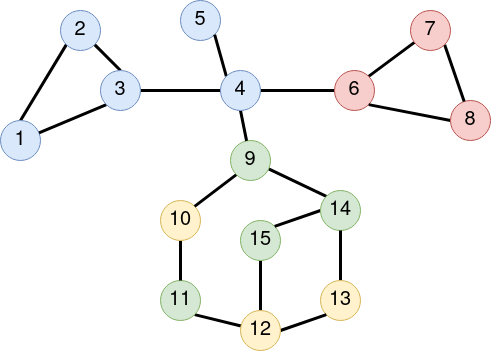
\includegraphics[width=.45\linewidth]{SLPARR5good.png}
    \label{fig:RR2}}
    \caption{Example Networks}
\end{figure}

\subsubsection*{Perfomance}
\begin{figure}[]
    \hspace*{-15pt}
    \centering
    \subfloat[Time in function of nodes]{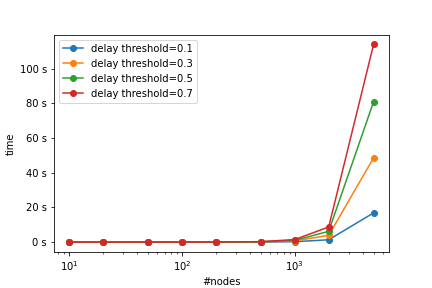
\includegraphics[width=.5\linewidth]{node.png}
    \label{fig:plotCommunity}}
    \subfloat[RR impact on performance]{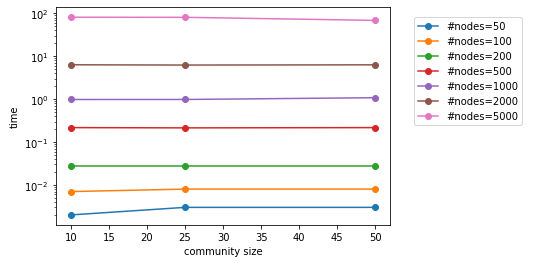
\includegraphics[width=.6\linewidth]{communitySize.png}
    \label{fig:plotSize}}
    \caption{Performance graphs}
\end{figure}

The performance of the SLPA algorithm has been measured locally outside the container, due to 
all the consideration done in the Functional Requirements section.
The following tests have been done in \textit{Ubuntu 18.04.4 LTS} on a \textit{AMD Ryzen 7 1700 Eight-Core}Processor.
\\
The algorithm has been tested on the following inputs: number of nodes in the network, delay threshold and maximum community size.
The number of nodes determines the size of the delay matrix. We tested networks with 10, 20, 50, 100, 200, 500, 1000, 2000 and 5000 nodes.
As previously said, the delay threshold is a constraint to which all cells of the delay matrix are subjected to. Every arc with and edge value grater than the delay threshold
is cancelled (the corresponding cell in the matrix is set to -1). We tested with the following thresholds: 0.1 , 0.3, 0.5, 0.7.
The maximum community size limits the number of nodes that can be in a community and we tested the same values reported in the PAPS testing phase
(10, 25, 50).\\
For each combination of these inputs a delay matrix is built. It's a $NxN$ matrix, where $N$ is the number of nodes in the network.
Every cell of the matrix has values between 0 and 1 drawn from a uniform probability distribution. In this way, the delay threshold
can be used to maintain a certain percentage of edges.
A delay threshold of 0.3 will roughly maintain the 30\% of the edges.
For each input a test is run ten times, tracking the execution time. In order to avoid noisy measurements,
the median of this values is considered instead of the mean.
\par
The figure \ref{fig:plotCommunity} plots the execution time in function of the number of nodes and delay threshold.
For small networks the algorithm runs in a few millisecond, and it manages to complete in about 10 seconds networks
with 1000 or 2000 nodes. SLPA starts to struggle with networks with 5000 nodes, starting to show an exponential trend.
\par
The figure \ref{fig:plotSize} highlights the fact that the maximum community size does not change the performance 
of the algorithm, because the total execution time is dominated by SLPA. This means that Round Robin does not
degrade performance, since its the only part of the algorithm affected by the community size, but just a constant cost regardless
of network size.